\documentclass[11pt, a4paper]{article}
\usepackage[utf8]{inputenc}
\usepackage[T1]{fontenc}
\usepackage{beton}
\usepackage{eulervm}
\usepackage{amsmath}
\usepackage{bm}
\usepackage{microtype}
\usepackage{ellipsis}
\usepackage{booktabs}
\usepackage{graphicx}
\usepackage{color}
\usepackage[hidelinks]{hyperref}
% \usepackage{siunitx}
%
%\usepackage[medium, compact]{titlesec}
%\usepackage[inline]{asymptote}
%\usepackage{tikz-cd}
\DeclareFontSeriesDefault[rm]{bf}{sbc}
% \usepackage{amssymb}
%% Turing grid is 21 columns (of 1cm if we are using A4)
%% Usually 4 "big columns", each of 4 text cols plus 1 gutter col;
%% plus an additional gutter on the left.
\usepackage[top=2.82cm, bottom=2.82cm, left=1cm, textwidth=11cm, marginparsep=1cm, marginparwidth=7cm]{geometry}
\usepackage[Ragged, size=footnote, shape=up]{sidenotesplus}
%% We used to use a two-column layout
% \setlength{\columnsep}{1cm}
\title{Automatic differentiation}
\author{James Geddes}
\date{\today}
%%
\newcommand{\eg}{\emph{Example:}}
\newcommand{\ie}{\emph{i.e.}}
\newcommand{\isdef}{\mathrel{\stackrel{\text{def}}{=}}}
\newcommand{\set}[1]{\boldmath{#1}}
\newcommand{\setR}{\set{R}}
\hyphenation{anti-sym-met-ric}
%%
% \usepackage[backend=biber]{biblatex}
% \addbibresource{../cyberdefence.bib}
% \DefineBibliographyStrings{english}{
%   andothers = {\mkbibemph{et\addabbrvspace{al}\adddot}}
% }
%%
\begin{document}
\maketitle

Suppose we are given functions $f\colon \setR^3 \to \setR$,
$g\colon \setR^2\to\setR$, and $h\colon \setR\to\setR$, in such a way that
we are able to evaluate these functions and their derivatives at any
value of their arguments. In addition, suppose we are given some
expression involving composititions of these functions; for example,
\begin{equation}
  F(x, y, z) = f(x, g(y, z), h(z)).
\label{eq:example}\end{equation}
The problem is to evaluate $F$ and \emph{its} derivatives at some
point.

What is an expression? It is either a variable, like $x$, or the name
of a function together with a list of arguments, which are also
expressions. That is, it is a tree, shown on the right in
figure~\ref{fig:expression}.
\begin{marginfigure}
  \centering
  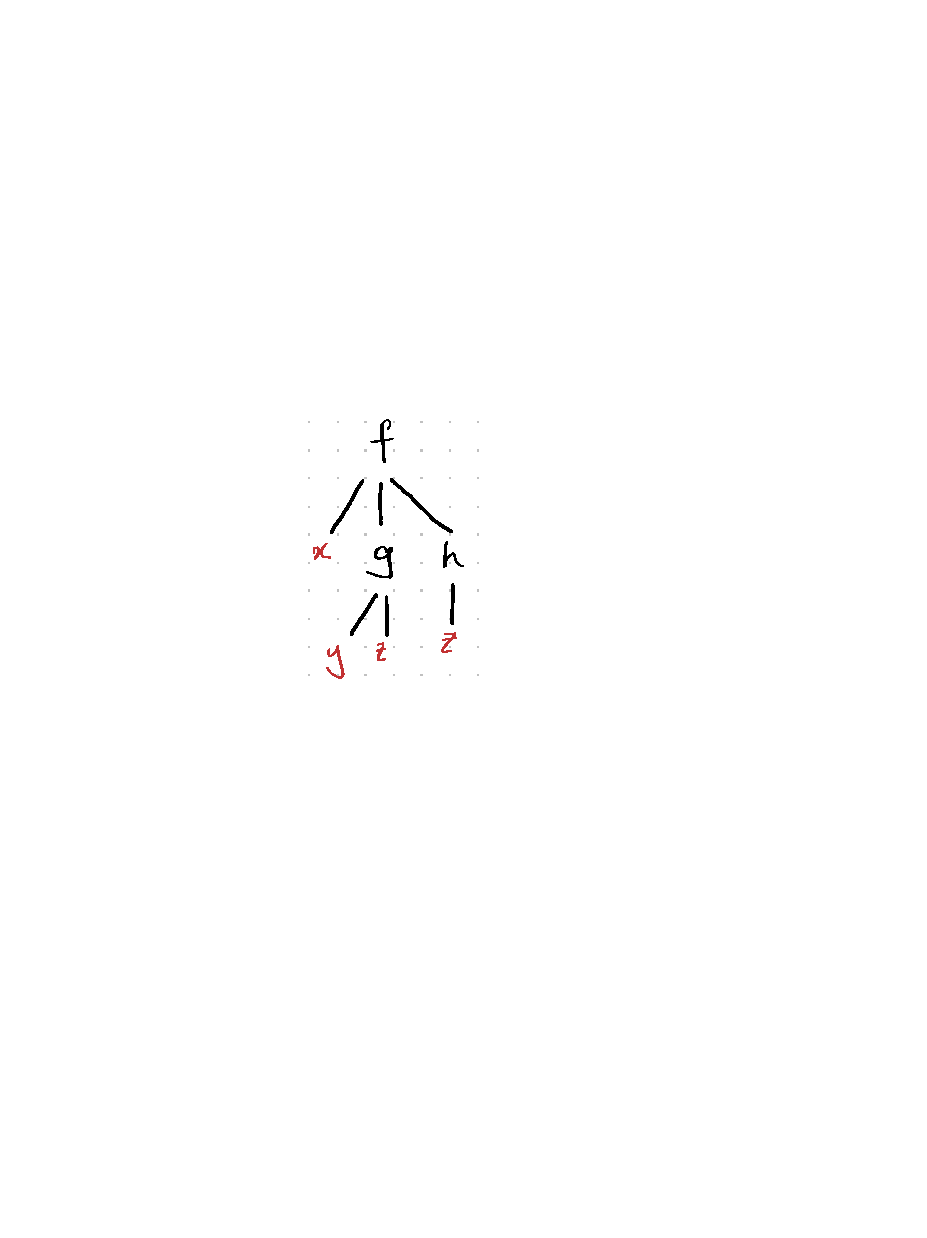
\includegraphics{images/expression.pdf}
  \caption{A tree, representing the expression $f(x, g(y, z), h(z))$.\label{fig:expression}}
\end{marginfigure}
An expression is either a \emph{variable}, like $x$, or the
\emph{application} of a function to its arguments, which are also
expressions. Note that there is a distinction, in
eq.~\eqref{eq:example}, between the names of functions (like $f$) and
the names of variables (like $x$). The function names are supposed to
refer to functions that are given to us in some way. The variable
names are merely placeholders to indicate which argument of $F$ is
being referred to. That is, the meaning of eq.~\eqref{eq:example}
would be unchanged if $x$ were replaced by $u$ everywhere; but its
meaning would be different if $f$ were replaced by $m$ everywhere.

Evaluating an expression is reasonably straightforward. To evaluate
an expression at a particular value of the variables:
\begin{enumerate}
\item If the expression is a variable, its value is the value of that
  variable;
\item Otherwise, the expression is a function application. Evaluate
  the arguments and then apply the function. 
\end{enumerate}

What about the derivative? For example, we may wish to evaluate
\begin{equation}
  \label{eq:partial-example}
  \frac{\partial F(x,y,z)}{\partial x}
\end{equation}
at some particular value of $x$, $y$, and~$z$. The ``chain rule'' is a
general theorem for computing the derivative of the composition of
functions. Suppose that $s$ and $t$ are functions of a single
variable. The chain rule is sometimes written as
\begin{equation*}
  \label{eq:chain-rule}
  \frac{d}{dx} s(t(x)) = \frac{d s}{dt} \frac{dt}{dx}. 
\end{equation*}

However, there is an abuse of notation here. Since $t$ is a function,
it is not clear what is meant by the term $ds/dt$, the derivative of
$s$ with respect to~$t$. What is really meant is ``the derivative of
$s$ with respect to its argument, evaluated at $t(x)$.''  The symbol
$t$ is being used both as a placeholder for the argument and as the
name of a function.

I shall use the following notation. For ``the derivative of $f$ with
respect to its $i$-th argument,'' I shall write $\partial_i f$. With this
notation, the chain rule would be written
\begin{equation}
  \label{eq:chain-rule}
  \frac{\partial F(x)}{\partial x} = (\partial_1s)(t(x)) \, \frac{\partial t}{\partial x}.
\end{equation}

The term $(\partial_1s)(t(x))$ means ``the derivative of the function $s$ with
respect to its first (and, in this example, only) argument, evaluated
at $t(x)$.''

The notation still isn't great. There are two many parentheses for one
thing. And $F(x)$ really ought to mean ``the value of the function $F$
at~$x$'' rather than, as we have used it here, ``the function $F$.''
Part of the problem is that $x$ is doing double duty: as the specific
location at which we are evaluating the derivative and as the variable
with respect to which we are taking the derivative. We shall try to
fix that later.

The chain rule extends to multivariate functions. The derivative of
$s(t(x,y),u(x,t))$ with respect to $x$ is
\begin{equation*}
  \frac{\partial }{\partial x} s\bigl(t(x,y),u(x,t)\bigr) =
  (\partial_1s) \frac{\partial t}{\partial x} 
  + (\partial_2s) \frac{\partial u}{\partial x},
\end{equation*}
and likewise for the derivative with respect to~$y$. In the above, it
is understood that $\partial_1s$, say, is to be thought of as a function of
$u$ and $t$, and evaluated at $u(x)$ and $t(x)$.

If, in the above example, $t$ and $u$ were themselves functions of
functions, then the chain rule applies recursively to
those.

Returning to eq.~\eqref{eq:example}, one obtains
\begin{equation*}
  \begin{aligned}
    \partial F / \partial x &= \partial_1 f, \\
    \partial F / \partial y &= \partial_2 f\,\frac{\partial g}{\partial y}, \\
    \partial F / \partial z &= \partial_2 f\,\frac{\partial g}{\partial z} 
                      + \partial_3f\,\frac{\partial h}{\partial z}. \\
  \end{aligned}
\end{equation*}

Many of the terms in the derivatives of $F$ are zero but the general
pattern is clear. In order to compute the derivative of $F$, one
constructs the same expression tree as in figure~\ref{fig:expression}
and recursively computes the derivatives of each node:
\begin{enumerate}
\item If the node is a variable, then its value is the value of that
  variable (as before) and its derivative with respect to some
  variable is either 0 (if the variables are different) or 1 (if they
  are the same). 
\item Otherwise, the node is a function application. Compute the values
  of the arguments, and the values of their derivatives. Now multiply
  the derivative of this function with respect to each of \emph{its}
  arguments by the corresponding derivative of the arguments, and sum. 
\end{enumerate}

The complete set of derivatives of $F$ can thus be computed in a
single, depth-first traversal of the tree. Say the expression graph
has $V$ nodes and $E$ edges. The cost of the original expression is
$O(V)$, since one performs one function evaluation for each node.
What is the computational cost of the derivative calculation?

Suppose we are compting the derivative with respect to some
variable,~$x$. Consider some node, $f$, encountered during the
calculation, having $n$ arguments. We must evaluate $f$, as before,
and in addition each of its derivatives,~$\partial_i f$ (for
$i=1,\dotsc,n$). Then there are $n$ multiplications of the
$\partial_i f$ with the $x$-derivative of the $i$-th argument (as well as the
sum).










\end{document}
